\documentclass[SDSUThesis.tex]{subfiles} 
\begin{document}

% new section
\section{CASE STUDY: SCORING AN SDO OF A LARGE FINANCIAL INSTITUTION}

    Data has been collected from the software development processes of
    an SDO within a large financial institution\footnote{All the raw data 
    files are available at \cite{Swanstrom2015}}.
    The data collection was from 2007 to January 2015. Only 4 elements had available
    data, and not all elements had data available for the entire time period.  The
    elements to be used are: quality, availability, schedule, and requirements.
    CRI is still effective when not all data is available.
    The overall CRI score will then be a 
    weighted average of the available elements. 
    This section will serve as a guide to preparing the CRI score
    based upon the available data.  

    \subsection{WITH HISTORICAL DATA}
        After the data has been collected, the raw data can be stored in the SDLC
        if desired.  Then scores for each of the 4 elements can be calculated.
        For this example, the value of $k$ will be 100 and the time
        frequency will be monthly.  Thus, scores will fall
        in the range $[-100,100]$.  Also, equal weighting is applied to 
        all elements and all Project IDs, Application IDs, and System IDs.
        \subsubsection{QUALITY}
            The first step to dealing with the quality data is a quick
            analysis of the data.  Table \ref{tab:quality_desc} provides
            some descriptive statistics for the quality data.  Testing hours
            were not capture but they are optional, so the analysis can 
            continue.
            
            
            \begin{longtable}{@{}l rr rrr}
                \toprule%
                 \centering%
                 {\bfseries Column}
                 & {\bfseries Min}
                 & {\bfseries Max}
                 & {\bfseries Median}
                 & {\bfseries Mean}
                 & {\bfseries Variance} \\
                
                \cmidrule[0.2pt](r{0.125em}){1-1}%
                \cmidrule[0.2pt](lr{0.125em}){2-2}%
                \cmidrule[0.2pt](l{0.125em}){3-3}%
                \cmidrule[0.2pt](l{0.125em}){4-4}%
                \cmidrule[0.2pt](l{0.125em}){5-5}%
                % \midrule
                \endhead
                
                Development Effort & 0 & 26937 & 300 & 1637 & 18383464 \\
                \myrowcolour%
                Testing Effort & NA & NA & NA & NA  & NA\\
                SIT Defects & 0 & 1106 & 1 & 45.86 & 24528 \\
                \myrowcolour%
                UAT Defects & 0 & 277 & 0 & 10.28 & 1306 \\
                PROD Defects & 0 & 1216 & 5 & 51.5 & 20311 \\
                
                \bottomrule
                
                \multicolumn{6}{c}{985 obs. from 23 Application IDs from 2007 to 2015} \\
                
                \caption{QUALITY DATA DESCRIPTIVE STATISTICS}
                \label{tab:quality_desc}
            \end{longtable}
            
            Notice, the data for quality goes from October 2007 to January 2015
            and contains 985 observations.
            This is important because historical data can be used to create the
            baseline quality function.  All quality for the years 2007 through 
            the end of 2013
            will be used as historical data for the purposes of creating
            the baseline quality function.  Once the historical data is separated,
            it results in 799 observations to be used for creating the baseline
            quality function.  Figure \ref{fig:quality-plots1} shows scatterplots
            of PROD\_DFTS versus the independent variables of DEV\_EFF, SIT\_DFTS,
            and UAT\_DFTS.  It can be seen that some correlations exist between
            the variables.
            
            \begin{figure}[ht]
                \centering
                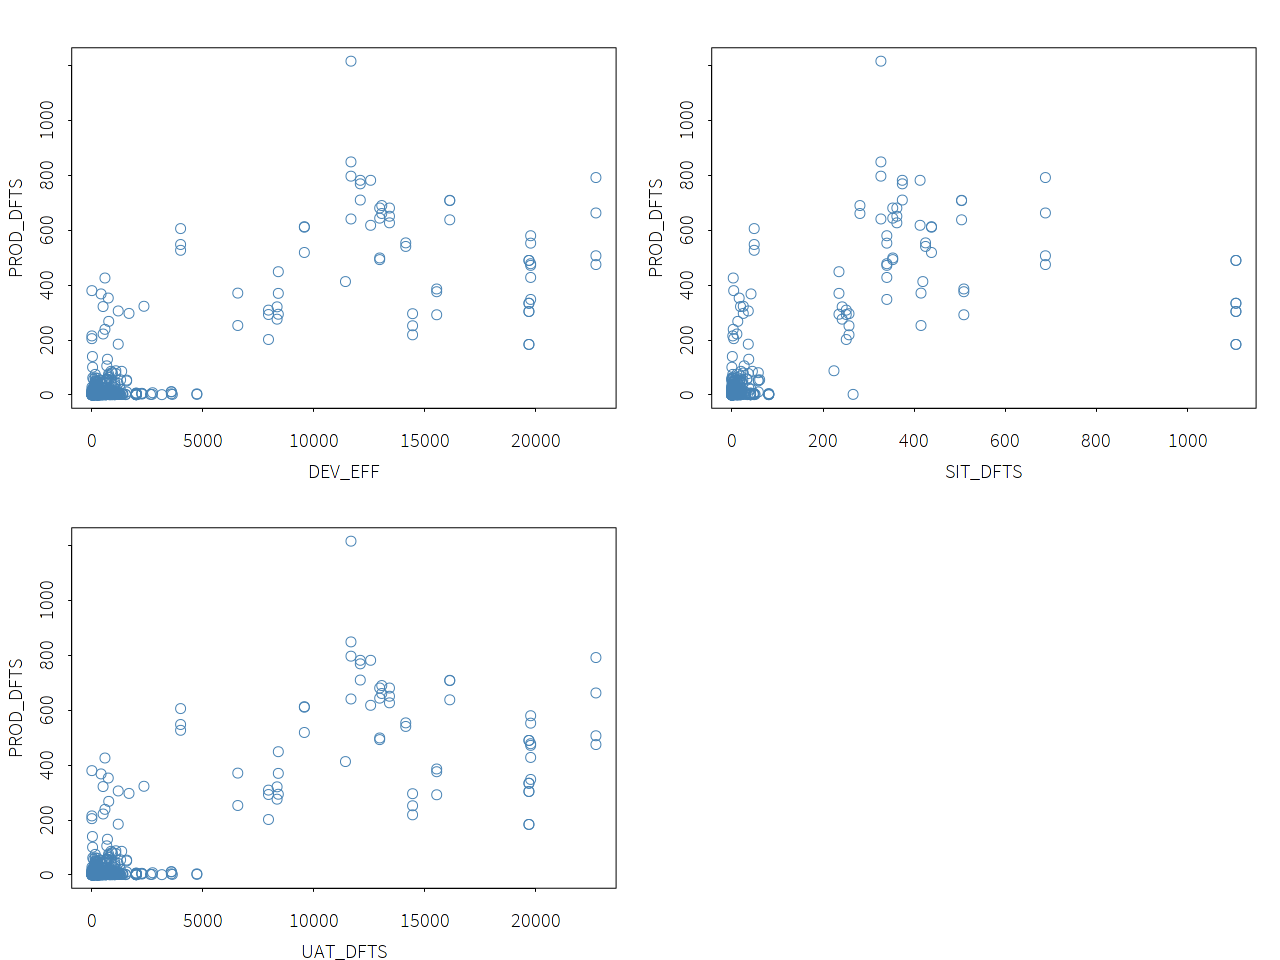
\includegraphics[scale=.3]{images/quality_plots1.png}
                \caption{QUALITY DATA PLOTS: DEPENDENT VS. INDEPENDENT VARIABLES}
                \label{fig:quality-plots1}
            \end{figure}
            
            Figure \ref{fig:quality-plots1} also shows the presence of a possible outlier
            with 1216 PROD\_DFTS.  That data point is dropped for the remaining analysis.
            At this point, a simple linear regression model can be fit to the remaining
            798 observations. At this point, no transformations have been performed
            on the data.  The linear regression model yields all 3 independent
            variables as significant and an overall $R^2 = .72$.  The source
            code and some further analysis can be found in Appendix 
            \ref{app:quality-history}. It appears to 
            be a good fit and thus all Application IDs will have the same baseline
            quality function.  Therefore, $f$ does not need a subscript, and $f$
            can be seen below.
            
            \[
                f = 5.92+ 0.035 \cdot DEV\_EFF - 0.36 \cdot SIT\_DFTS + 1.05 \cdot UAT\_DFTS
            \]
            
            Now that $f$ has been determined, the quality scores for each
            application can be calculated for all the months beyond 2013.
            Appendix \ref{src:quality} provides the necessary R code to
            perform the calculations.  Figure \ref{fig:quality-scores} shows
            the quality scores for 2014 and beyond.  As can be seen, the
            scores are greatly above expectations.  That is an indication
            of improved quality over historical performance.
            
            \begin{figure}[ht]
                \centering
                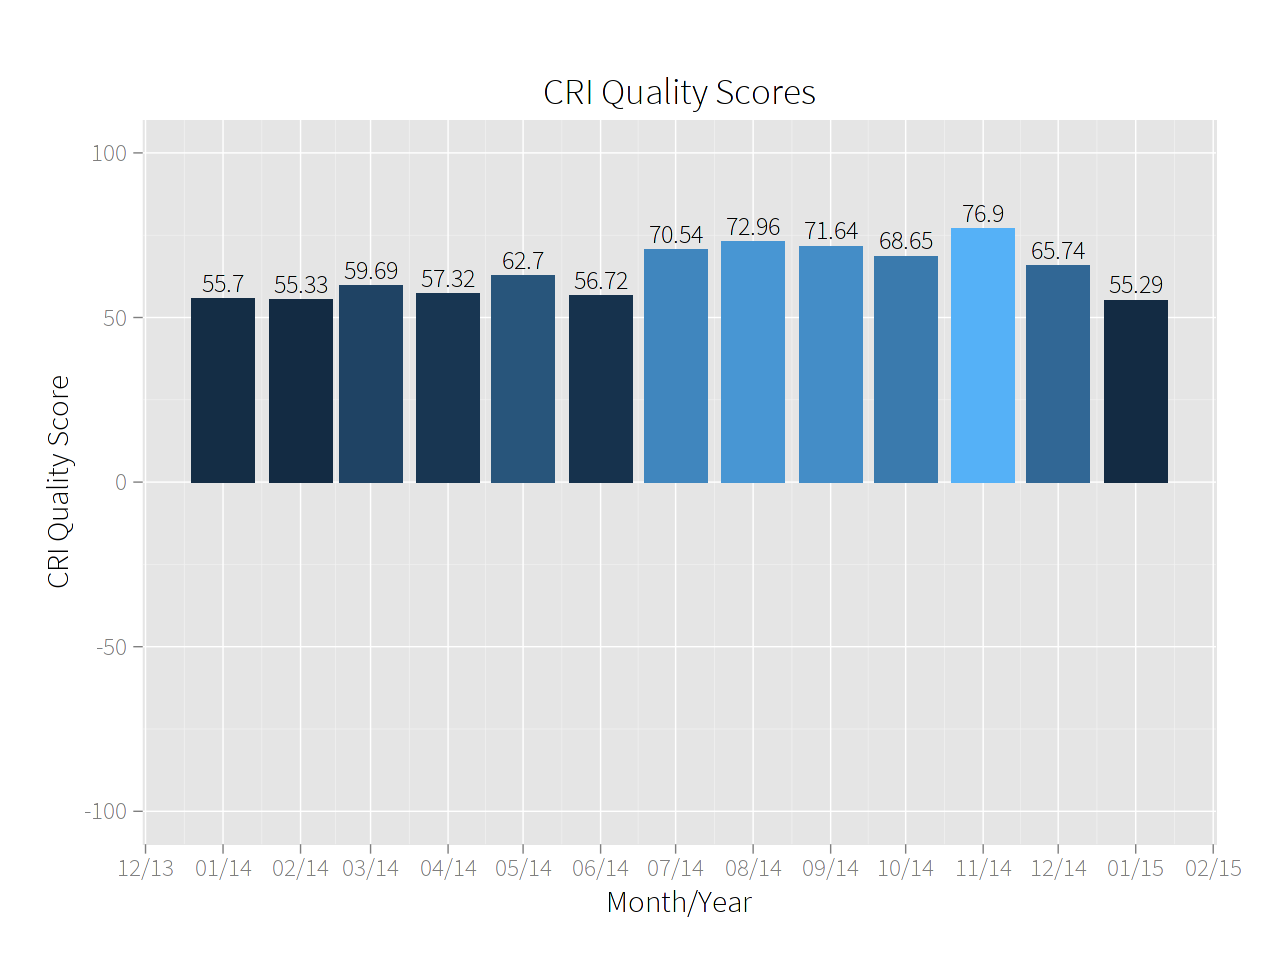
\includegraphics[scale=.3]{images/quality_scores.png}
                \caption{CRI QUALITY SCORES}
                \label{fig:quality-scores}
            \end{figure}
            
            
            
            
        \subsubsection{AVAILABILITY}
            For the availability data,
            some descriptive statistics can be seen in 
            Table \ref{tab:availability_desc}.  The percent uptime
            was precalculated for this data so uptime, scheduled downtime,
            and unscheduled downtime are not needed.  Availability
            does not rely upon analysis of historical data since
            a known upper and lower bound exist, 1 and 0 respectively.
            
            \begin{longtable}{@{}l rr rrr}
                \toprule%
                 \centering%
                 {\bfseries Column}
                 & {\bfseries Min}
                 & {\bfseries Max}
                 & {\bfseries Median}
                 & {\bfseries Mean}
                 & {\bfseries Variance} \\
                
                \cmidrule[0.2pt](r{0.125em}){1-1}%
                \cmidrule[0.2pt](lr{0.125em}){2-2}%
                \cmidrule[0.2pt](l{0.125em}){3-3}%
                \cmidrule[0.2pt](l{0.125em}){4-4}%
                \cmidrule[0.2pt](l{0.125em}){5-5}%
                % \midrule
                \endhead
                
                Percent Uptime & 0 & 1.0 & 1.0 & 0.9745 & 0.023 \\
                \myrowcolour%
                Expected Percent Uptime & 0.93 & 1.0 & 0.98 & 0.9769  & 0.977\\
                
                \bottomrule
                
                \multicolumn{6}{c}{7522 obs. from 83 Application IDs from 2008 to 2015} \\
                
                \caption{AVAILABILITY DATA DESCRIPTIVE STATISTICS}
                \label{tab:availability_desc}
            \end{longtable}
            
            Since percent uptime has already been calculated and no historical
            analysis needs to be performed, the calculation of the scores
            can be performed. 
            R code to compute the CRI availability scores can be found in Appendix
            \ref{src:availability}. Figure \ref{fig:availability-scores} displays
            the CRI availability scores.  As can be seen the scores are all above
            70.  That is good from a performance standpoint, but it might be an
            indication that the expected uptimes could be raised.  If expected
            uptimes are consistently being exceeded, some consideration should
            be given to increase the expected uptimes.  This shows that
            organizations, or at least this particular organization, are getting
            very good at keeping computer systems available.  Therefore,
            SLAs need to be adjusted to properly reflect the better performance.
            
            \begin{figure}[ht]
                \centering
                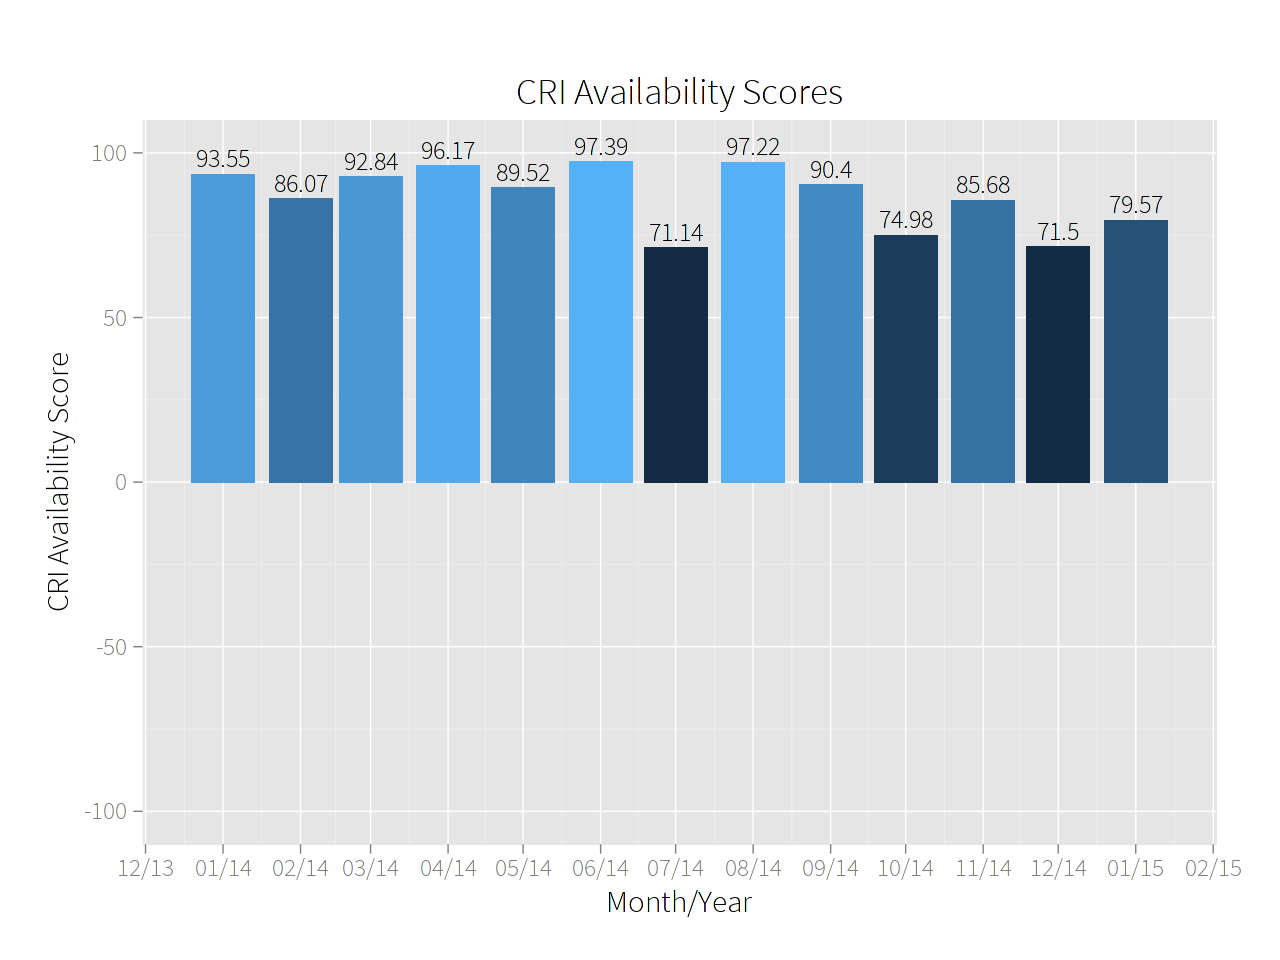
\includegraphics[scale=.3]{images/availability_scores.png}
                \caption{CRI AVAILABILITY SCORES}
                \label{fig:availability-scores}
            \end{figure}
            
            
            
            
            
        \subsubsection{SCHEDULE}
        \subsubsection{REQUIREMENTS}
            There were 15 rows of data that contained 0 for both
            scheduled and actual
            \begin{longtable}{@{}l rr rrr}
                \toprule%
                 \centering%
                 {\bfseries Column}
                 & {\bfseries Min}
                 & {\bfseries Max}
                 & {\bfseries Median}
                 & {\bfseries Mean}
                 & {\bfseries Variance} \\
                
                \cmidrule[0.2pt](r{0.125em}){1-1}%
                \cmidrule[0.2pt](lr{0.125em}){2-2}%
                \cmidrule[0.2pt](l{0.125em}){3-3}%
                \cmidrule[0.2pt](l{0.125em}){4-4}%
                \cmidrule[0.2pt](l{0.125em}){5-5}%
                % \midrule
                \endhead
                
                Scheduled & 0 & 1.0 & 1.0 & 0.9745 & 0.023 \\
                \myrowcolour%
                Expected Percent Uptime & 0.93 & 1.0 & 0.98 & 0.9769  & 0.977\\
                Expected Percent Uptime & 0.93 & 1.0 & 0.98 & 0.9769  & 0.977\\
                
                \bottomrule
                
                \multicolumn{6}{c}{476 obs. from 402 Project IDs from 2010 to 2015} \\
                
                \caption{REQUIREMENTS DATA DESCRIPTIVE STATISTICS}
                \label{tab:requirements_desc}
            \end{longtable}
            
        \subsubsection{OVERALL}
            All of the months do not include the same elements.  
    
    An CRI calculation analyzing historical performance.

%%\subsection{WITHOUT HISTORICAL DATA}

%%An CRI calculation with default values for quality, schedule and requirements.

\end{document}